\ifx\mainfile\undefined
%  ========================================================================
%  Copyright (c) 2006-2011 The University of Washington
%
%  Licensed under the Apache License, Version 2.0 (the "License");
%  you may not use this file except in compliance with the License.
%  You may obtain a copy of the License at
%
%      http://www.apache.org/licenses/LICENSE-2.0
%
%  Unless required by applicable law or agreed to in writing, software
%  distributed under the License is distributed on an "AS IS" BASIS,
%  WITHOUT WARRANTIES OR CONDITIONS OF ANY KIND, either express or implied.
%  See the License for the specific language governing permissions and
%  limitations under the License.
%  ========================================================================
%
 
\documentclass [11pt, twoside] {uwthesis}

\usepackage{color}
\usepackage{url}
\usepackage{amsmath}
\usepackage{amsfonts}
\usepackage[bookmarks,
	hidelinks,
	plainpages=false,
	pdfpagelabels,
	pagebackref=true,
            ]{hyperref}
\renewcommand*{\backref}[1]{}% for backref < 1.33 necessary
\renewcommand*{\backrefalt}[4]{%
  \ifcase #1 %
    (No citations.)%
  \or
    (Cited on page #2.)%
  \else
    (Cited on pages #2.)%
  \fi
}

\newcommand{\biburl}[1]{{\tt<}\url{#1}{\tt>}}

\hypersetup{%
pdfauthor = {Daniel Chaim Halperin},
pdftitle = {Simplifying the Configuration of 802.11 Wireless Networks with Effective SNR},
pdfsubject = {Ph.D. Dissertation},
pdfkeywords = {},
pdfcreator = {University of Washington, Computer Science and Engineering},
pdfproducer = {},
bookmarksopen = {true},
pdfpagelayout = {TwoColumnRight},
}

\usepackage{footnotebackref}
%%%%%%%%%%%%%%%%%%%%%%%%%%%%%%%%%%%%%%%%%%%%%%%%%%%%%%
%%%        Formatting sections                     %%%
%%%%%%%%%%%%%%%%%%%%%%%%%%%%%%%%%%%%%%%%%%%%%%%%%%%%%%
\newcommand{\algref}[1]{Algorithm~\ref{#1}}
\newcommand{\chapref}[1]{Chapter~\ref{#1}}
\renewcommand{\eqref}[1]{Equation~\ref{#1}}
\newcommand{\figref}[1]{Figure~\ref{#1}}
\newcommand{\secref}[1]{\S\ref{#1}}
\newcommand{\tabref}[1]{Table~\ref{#1}}
\newcommand{\heading}[1]{\vspace{4pt}\noindent\textbf{#1}}
\newcommand{\topheading}[1]{\noindent\textbf{#1}}
\newcommand{\noheading}[0]{\vspace{4pt}\noindent}

%%%%%%%%%%%%%%%%%%%%%%%%%%%%%%%%%%%%%%%%%%%%%%%%%%%%%%
%%%        XXX and other warnings                  %%%
%%%%%%%%%%%%%%%%%%%%%%%%%%%%%%%%%%%%%%%%%%%%%%%%%%%%%%
\newcommand{\xxx}[1]{\textit{\color{red}XXX #1}}

%%%%%%%%%%%%%%%%%%%%%%%%%%%%%%%%%%%%%%%%%%%%%%%%%%%%%%
%%%        Units                                   %%%
%%%%%%%%%%%%%%%%%%%%%%%%%%%%%%%%%%%%%%%%%%%%%%%%%%%%%%
\usepackage{xspace}
\newcommand{\unitsep}{\texorpdfstring{\,}{ }}
\def\unit#1{% from: http://www.tex.ac.uk/cgi-bin/texfaq2html?label=csname "Defining a macro from an argument"
  \expandafter\def\csname #1\endcsname{\unitsep\text{#1}\xspace}%
}
\def\varunit#1#2{% from: http://www.tex.ac.uk/cgi-bin/texfaq2html?label=csname "Defining a macro from an argument"
  \expandafter\def\csname #1\endcsname{\unitsep\text{#2}\xspace}%
}
\unit{GHz}
\unit{MHz}
\unit{kHz}
\unit{Gbps}
\unit{Mbps}
\unit{KB}
\unit{dB}
\unit{dBi}
\unit{dBm}
\unit{W}
\unit{mW}
\varunit{uW}{$\mu$W}
\unit{ms}
\varunit{us}{$\mu$s}
\unit{h}
\unit{m}
\unit{s}
\unit{km}
\unit{cm}
\unit{mm}
\varunit{mmsq}{mm$^\text{2}$}
\varunit{insq}{in$^\text{2}$}
\newcommand{\degree}{\ensuremath{^\circ}\xspace}
\newcommand{\degrees}{\degree}
%%%%%%%%%%%%%%%%%%%%%%%%%%%%%%%%%%%%%%%%%%%%%%%%%%%%%%%%%%%%%%%%%%%%%%%%%%%%%%%%%%%%%%
% Euler for math | Palatino for rm | Helvetica for ss | Courier for tt
%
% From: http://www.tug.org/mactex/fonts/LaTeX_Preamble-Font_Choices.html
%%%%%%%%%%%%%%%%%%%%%%%%%%%%%%%%%%%%%%%%%%%%%%%%%%%%%%%%%%%%%%%%%%%%%%%%%%%%%%%%%%%%%%
\renewcommand{\rmdefault}{ppl} % rm
\usepackage[scaled]{helvet} % ss
\usepackage{courier} % tt
\usepackage{eulervm} % a better implementation of the euler package (not in gwTeX)
\normalfont
\usepackage[T1]{fontenc}
%%%%%%%%%%%%%%%%%%%%%%%%%%%%%%%%%%%%%%%%%%%%%%%%%%%%%%%%%%%%%%%%%%%%%%%%%%%%%%%%%%%%%%

%%%%%%%%%%%%%%%%%%%%%%%%%%%%%%%%%%%%%%%%%%%%%%%%%%%%%%
%%%        Figures                                 %%%
%%%%%%%%%%%%%%%%%%%%%%%%%%%%%%%%%%%%%%%%%%%%%%%%%%%%%%
\usepackage{graphicx}
% Caption package both lets you set the spacing between figure and caption
% and also makes the \figref{} point to the right place.
\usepackage[font=bf,aboveskip=6pt,belowskip=-4mm]{caption}
% Allow subfigures, make them bold
\usepackage[bf,BF,small]{subfigure}
% List of figures
\setcounter{lofdepth}{2}  % Print the chapter and sections to the lot

%%%%%%%%%%%%%%%%%%%%%%%%%%%%%%%%%%%%%%%%%%%%%%%%%%%%%%
%%%        Lists with reduced spacing              %%%
%%%%%%%%%%%%%%%%%%%%%%%%%%%%%%%%%%%%%%%%%%%%%%%%%%%%%%
\usepackage{enumitem}

%%%%%%%%%%%%%%%%%%%%%%%%%%%%%%%%%%%%%%%%%%%%%%%%%%%%%%
%%%        Fancy tables                            %%%
%%%%%%%%%%%%%%%%%%%%%%%%%%%%%%%%%%%%%%%%%%%%%%%%%%%%%%
\usepackage{tabulary}
\usepackage{booktabs}

%%%%%%%%%%%%%%%%%%%%%%%%%%%%%%%%%%%%%%%%%%%%%%%%%%%%%%
%%%        Formatting techniques/tools/etc.        %%%
%%%%%%%%%%%%%%%%%%%%%%%%%%%%%%%%%%%%%%%%%%%%%%%%%%%%%%
\newcommand{\term}[1]{\texttt{#1}}

\begin{document}
 
\textpages
\setcounter{chapter}{5} % Set to n-1!
\fi
%%%%%%%%%%%%%%%%%%%%%%%%%%%%%%%%%%

\cleardoublepage
\chapter{Evaluating Effective SNR for MIMO-OFDM Channels}
\label{chap:delivery}

In this chapter, I experimentally evaluate how well my Effective SNR model predicts packet delivery for 802.11n wireless links. This is the fundamental measure of whether the model can be useful; good predictions are necessary to properly configure links and networks to solve the link and network configuration problems.

To do so, I use my CSI measurement tool to gather a wide range of channel and performance information across 200 wireless links in both testbeds. This captures a wide variety of fading environments, from line-of-sight links in the same room to links between nodes in different rooms with RF barriers and reflectors spread around and between them. I use this data to evaluate the accuracy of predictions made using Packet SNR and Effective SNR.

The primary study in this chapter determines how accurately Effective SNR predicts whether packets will be delivered using different modulation and coding schemes. The goal is that for every MCS, a clear Effective SNR threshold separates those links that do not deliver packets at that rate from those that do, and thus that my model is accurate for practical links. I also compare how well Packet SNR works when used in the same way.

I next consider how well my model enable predictions about the effects of transmit power control on rate. This joint optimization problem highlights my model's flexibility. I conclude this chapter by evaluating the resilience of my Effective SNR system to interference, so that it can still be used to make predictions in contested wireless environments.

Combined, these three studies lay the foundation for showing that Effective SNR is accurate, flexible, and practical. In subsequent chapters I deploy my model as part of a system in the context of many application-related configuration problems.

\section{Experimental Data}
I measured packet delivery over a 20\MHz channel on my two 802.11n testbeds, using links with four different antenna configurations:
\begin{enumerate}[parsep=1ex,itemsep=1ex,topsep=1ex]
\item The \textbf{SISO} configuration uses a single antenna at each node. This configuration corresponds to 802.11a.
\item The \textbf{SIMO} configuration uses a single transmit antenna but three receive antennas. This is an 802.11a/g/n configuration that uses spatial diversity techniques.
\item The \textbf{MIMO2} configuration uses two spatial streams and three receive antennas. This employs both 802.11n techniques of spatial multiplexing and spatial diversity.
\item The \textbf{MIMO3} configuration uses three antennas at each node to send and receive three spatial streams. This configuration uses spatial multiplexing, but does not additionally benefit from spatial diversity.
\end{enumerate}

For each of these configurations, I measured the packet delivery for each link using each MCS, at at each transmit power level between $-$10\dBm and $+$16\dBm in steps of 2\dB. I sent 1,500-byte packets as constant bit-rate UDP traffic generated by \program{iperf} at 2\Mbps for 5 seconds, about 860 packets total. The receiver also recorded the CSI and per antenna RSSIs and noise floors to measure the RF channel for each correctly received packet. In these experiments, I turned off 802.11's link layer retransmissions in order to observe the underlying packet delivery rate. The experiments were conducted at night on unused 802.11 channels in order to minimize the effects of environmental movement and RF interference on these results.

%Note that CSI and RSSI are measured during the preamble, and so do not depend on the transmit rate, though they vary with the number of streams. 
%Similarly, 3x3 CSI gives us the channel between each pair of transmit and receive antennas, so it also implicitly contains 1x1 CSI.

The above testing gives ground truth data to probe variation across 200 links, 26\dB of transmit power, four antenna configurations ranging from SISO to MIMO3, and 8 MCS values per configuration. This covers all of the key variables needed to implement and evaluate my Effective SNR model.

\section{Packet Delivery with Effective SNR}
The first study in this chapter aims to understand whether Effective SNR is a good metric, i.e., whether it is an accurate predictor of packet delivery. In this section, I evaluate the model in two ways. The first is via the \define{transition window}, i.e., the SNR regime in which packet delivery for all links goes from near-zero to near-perfect. We saw in \chapref{chap:problem} that this transition occurs rapidly for a wired link (\figref{fig:snr_prr_attenuator}), but occurs over a wide range for wireless links (\figref{fig:snr_prr_26_65}) when using the Packet SNR. A narrow transition window would be one indicator that Effective SNR works well.

The second evaluation metric is \define{rate confusion}, i.e., how many rates might be best at a particular SNR value. The example wired link showed clear separation between rates, such that at every SNR value there is a clear best rate. Conversely, because the transition regions of different wireless links overlap, links with the same Packet SNR might support very different rates. 

For both analyses, I evaluate the predictions made by my Effective SNR model independently and as compared to Packet SNR.

\subsection{Transition Windows}
I begin with a visual comparison of the transition regions for real wireless links, and then present a quantitative evaluation of the difference between Packet SNR and Effective SNR in transition window width. I focus on SISO links, for which the most testbed links transition from being lossy to reliable. I examine the remaining configurations in the next section.

\begin{figure}[t!]
	\centering
	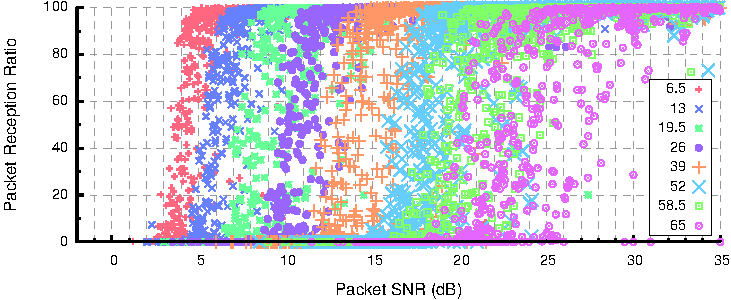
\includegraphics[width=\textwidth]{figures/delivery_figures/snr_prr_scatter_siso.pdf}
	\caption[SNR vs PRR for all SISO modulations]{\label{fig:snr_prr_siso} A scatterplot of Packet SNR versus PRR for real wireless links shows wide transition regions and significant overlap between rates.}
\end{figure}
\begin{figure}[t!]
	\centering
	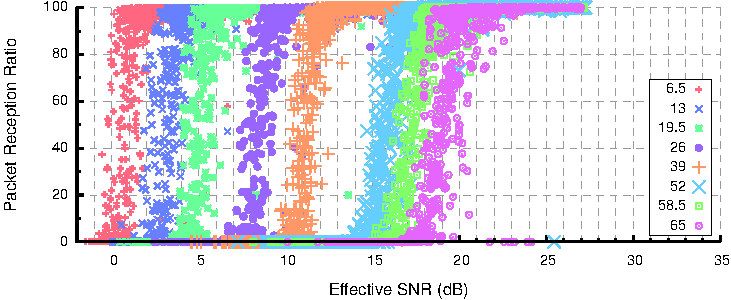
\includegraphics[width=\textwidth]{figures/delivery_figures/esnr_prr_scatter_siso.pdf}
	\caption[Effective SNR vs PRR for all SISO modulations]{\label{fig:esnr_prr_siso}Using the Effective SNR instead of Packet SNR reveals narrower transition regions and cleaner separation between rates. The overlap that is present is generally between links that use the same modulation but different coding schemes.}
\end{figure}

\subsubsection{Visual Comparison}
Recall \figref{fig:snr_prr_26_65} from \chapref{chap:problem}, which showed a scatterplot of Packet SNR versus Packet Reception Ratio (PRR) for three sample single-antenna modulations. This graph demonstrated that for real wireless links, the width of the transition region is 10\dB or more, so that there is a large range of power levels for which performance is unpredictable in practice.

In \figref{fig:snr_prr_siso}, I present a version of that plot for real SISO links that now includes data points for all eight modulation and coding schemes (MCSes). In this graph, we can see that there is a correlation between Packet SNR and rate, but also a significant overlap between rates. For most MCSes, the transition region is at least five and often ten dB wide. We see that for a large SNR range, many links will be lossy using one MCS, while other links will work well at the next higher, or even the second higher, rate. This explains why Packet SNR computed from RSSI does not provide a good indicator of performance in practice.

Contrast this figure with \figref{fig:esnr_prr_siso}, which shows the exact same set of data points but using Effective SNR instead of Packet SNR along the $x$-axis. This picture now shows a much clearer separation between rates. Especially for lower MCS values, only a few outlier links overlap with the next higher rate. Note also that, as shown in \chapref{chap:model}, the Effective SNR is several decibels lower than the Packet SNR because it measures the amount of power that is actually harnessed by the link, rather than the total power.

In both graphs the separation is generally larger between rates that use different modulations, e.g.\ between \mcs{2}, which uses QPSK, and \mcs{3}, which uses 16-QAM. In contrast, MCS that only differ in coding rate overlap to a more substantial degree. This effect is worst for the highest rates (\mcs{5}--\mcs{7}), which use 64-QAM modulation. I believe this artifact is fundamental, as it matches the results from the wired link (\figref{fig:snr_prr_attenuator}); I attribute it to the fact that these three MCS use coding rates 2/3, 3/4, and 5/6 that are much closer together than the 1/2-coded and 3/4-coded combinations used for the QPSK and 16-QAM rates.

\subsubsection{Quantitative Evaluation}
The visual comparison presented above shows qualitatively that Effective SNR provides a more compact transition region and clearer separation between rates, but note that scatterplots can be misleading because they obscure density and distributions---each plot above has 16,188 points. To understand the data qualitivately, I analyzed the SISO measurements to find the transition window for each of the measured links.

Formally, I define the transition window a particular rate to be the set of SNR values between which packet delivery rises from 10\% (lossy) to 90\% (reliable) for any link. \tabref{tab:transitions} gives the width of the transition window (denoted $\Delta\rho$) for SISO rates using the Packet SNR and Effective SNR metrics. I show the 25\%--75\% range of points in the transition window as a measure of the typical link, and the 5\%--95\% range as a measure of most links. A good result here is a narrow window like that measured over a wire (\figref{fig:snr_prr_attenuator}).

The table shows that the transition widths are consistently tight with my model. Most links transition within a window of around 2\dB for most rates. The width of the SNR-based transition windows is typically two to three times looser, especially for the denser modulation schemes like 64-QAM and higher code rates. This means that it is easy for a less than ideal channel to degrade the reception of high rates. However, while the transitions for the last four rates are inflated with SNR, they remain tight with Effective SNR.

\subsubsection{Limits on Accuracy}
In \tabref{tab:transitions}, the transition regions for Effective SNR range from 1\dB to about 3\dB, depending on MCS. In fact, these results for Effective SNR are about the best that can be obtained because they are close to textbook transitions for flat-fading channels and those measured over a wire (\figref{fig:snr_prr_attenuator}). A small improvement is surely possible, but this is probably limited by the precision of my measurement data. The IWL5300 gives RSSI, AGC and noise values in dB to the nearest integer, and at most 8-bit CSI over a 48\dB range for only 30 out of 56 subcarriers. With this combination of factors, quantization error of at least 1\dB is likely.

\subsubsection{Summary}
This section showed that my Effective SNR model provides a channel metric that can narrow transition windows and a separation between rates. The larger significance of narrow transition windows is that, by reducing them enough that they do not overlap, I can unambiguously predict the highest rate that will work for nearly all links nearly all of the time. In contrast, Packet SNR transition windows overlap such that for a given SNR there may be five different best rates across links the testbed. I explore this next.

\begin{table}
\centering
\begin{tabular}{cccccc}
\toprule
\multirow{2}{*}{MCS} & \multirow{2}{*}{Rate (Mbps)} & \multicolumn{2}{c}{$\Delta\rho_{\text{packet}}$ (dB)} &
\multicolumn{2}{c}{$\Delta\rho_{\text{eff}}$ (dB)} \\ 
\cmidrule(lr){3-4} \cmidrule(lr){5-6}
& &  ~~5\%--95\% & ~25\%--75\% & ~~5\%--95\% & ~25\%--75\%  \\
\midrule 
0 &  6.5                    & 3.08  & 1.29  & 2.05  & 0.81 \\
1 & 13.0                    & 3.45  & 1.44  & 2.38  & 0.89 \\
2 & 19.5                    & 6.27  & 3.12  & 2.30  & 0.85 \\
3 & 26.0                    & 3.93  & 1.98  & 3.02  & 0.94 \\
4 & 39.0                    & 7.05  & 3.49  & 2.19  & 0.93 \\
5 & 52.0                    & 7.16  & 3.20  & 2.29  & 1.06 \\
6 & 58.5                    & 7.25  & 3.37  & 2.92  & 1.41 \\
7 & 65.0                    & 7.24  & 2.81  & 2.92  & 1.35 \\
\midrule
\multicolumn{2}{c}{Average} & 5.68  & 2.59  & 2.51  & 1.03 \\         
\bottomrule
\end{tabular}
\caption[Width of SISO transition windows]{\label{tab:transitions} Width of SISO transition windows.}
\end{table}

%%%%%%%%%%%%%%%%%%%%%%%%%%%%%%%%%%%%%%%%%%%%%%%%%%%%%%%%%%%%%%%%%%%%%%%%%%%%%%%%%%%%%%%
\subsection{Rate Confusion}
\label{sec:rate_confusion}

\begin{figure}[p]
	\begin{leftfullpage}
	\centering
	\subfigure[SISO configurations]{
		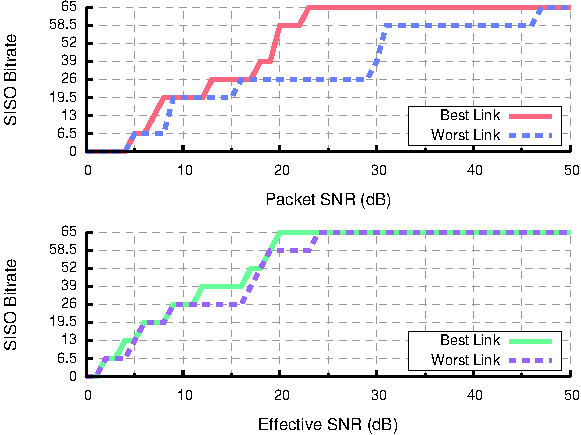
\includegraphics[width=0.8\textwidth]{figures/delivery_figures/siso_rate_confusion.pdf}%
		\label{fig:snr_rate_step_1x1}%
	}%
	
	\subfigure[SIMO configurations]{
		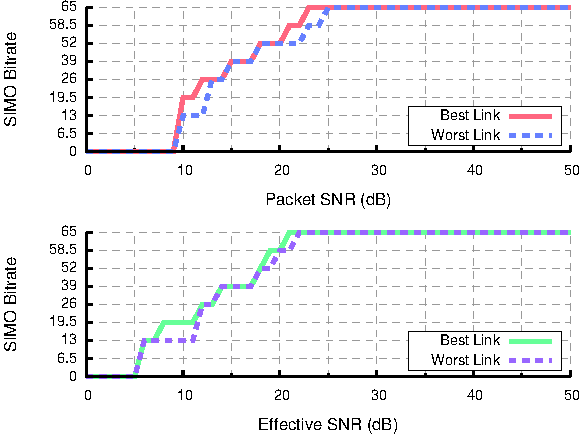
\includegraphics[width=0.8\textwidth]{figures/delivery_figures/simo_rate_confusion.pdf}%
		\label{fig:snr_rate_step_1x3}%
	}
	\caption[Rate confusion with Packet SNR and Effective SNR for different antenna configurations]{\label{fig:snr_rate_steps}Rate confusion with Packet SNR and Effective SNR. Excepting very low and high SNRs, one Packet SNR value maps to multiple best rates for different links. For the same data, 
Effective SNR provides a clear indicator of the best rate for nearly all links.}
	\end{leftfullpage}
\end{figure}

\setcounter{figure}{0}
\begin{figure}
\begin{xtrafullpage}
	\centering	
	\setcounter{subfigure}{2}
	\subfigure[MIMO2 configurations]{
		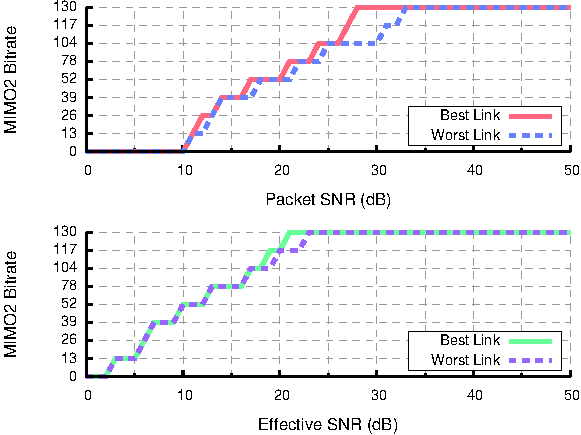
\includegraphics[width=0.8\textwidth]{figures/delivery_figures/mimo2_rate_confusion.pdf}%
		\label{fig:snr_rate_step_2x3}%
	}%

	\subfigure[MIMO3 configurations]{
		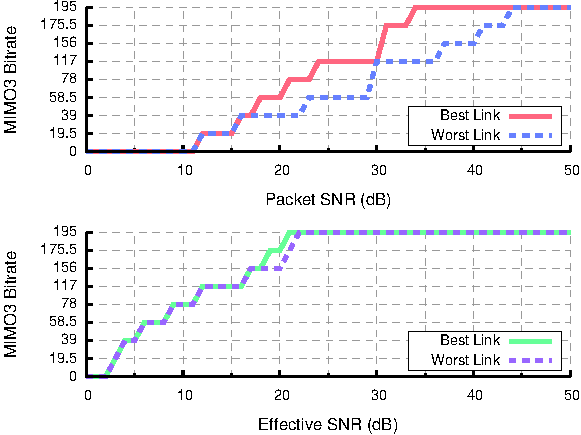
\includegraphics[width=0.8\textwidth]{figures/delivery_figures/mimo3_rate_confusion.pdf}%
		\label{fig:snr_rate_step_3x3}%
	}
	\vspace{36pt}
\end{xtrafullpage}
\end{figure}

To understand whether the Effective SNR model accurately predicts packet delivery, I analyze the fastest working rate (PRR$\geq$ 90\%) for each link and all NIC settings. \figref{fig:snr_rate_steps} shows the results broken down by configuration. The SISO experiment (\figref{fig:snr_rate_step_1x1}) shows links for both testbeds combined. The remaining graphs \figref{fig:snr_rate_step_1x3}--\ref{fig:snr_rate_step_3x3}  show rates for SIMO, MIMO2 and MIMO3 configurations for the Intel testbed only; it is denser than UW and supports MIMO experiments over our NIC's transmit power range.

These graphs study rate confusion, i.e., the ability of a given SNR value to predict the best rate across a wide set of links. If we consider the fastest rate each link supports at a particular Packet SNR or Effective SNR value, the best link is the link that supports the fastest rate, and the worst link is the slowest. The difference between the best and worst links, i.e., the set of possible best rates for an arbitrary link with a particular SNR, is the rate confusion. I plot this spread in these graphs. Note that the SIMO figure does not include data for the lowest 6.5\Mbps rate, because very few links experience loss at that rate within the transmit power range of the IWL5300---the added spatial diversity makes most links work well, as described below.

Ideally, the best and worst lines would overlap completely, such that the highest rate for a given SNR would be the same for the best and worst links. This rate would then be an accurate prediction for the particular Effective SNR or Packet SNR level. Conversely, gaps between the best and worst lines expose confusion about which MCS will yield the highest performance for that SNR.

For the SISO (\figref{fig:snr_rate_step_1x1}) and MIMO3 (\figref{fig:snr_rate_step_3x3}) cases, the figures show that using Packet SNR results in a large spread between the best and worst lines. Except for extremely low and high SNRs, nearly all SNRs have at least two---and up to five different---rates as suitable choices for the best rate. That is, Packet SNR often poorly indicates rate.

In sharp contrast, %looking at bottom lines in the graphs, 
the two Effective SNR lines overlap almost all the time, and mostly appear to be a single line. This is almost an ideal result. Effective SNR is a clear indicator of best rate. When there is slight separation, the spread is only between rates that use the same modulation but different amounts of coding, just as I described in the last section. These combinations are also close together in our wired experiments. 

Interestingly, these results show that Packet SNR predictions are much better for the SIMO and MIMO2 cases, though still not as accurate as Effective SNR, particularly for the highest rates. The reason is \emph{spatial diversity}: spare receive antennas gather the received signal and combine to make the channel more frequency-flat, thus bringing the Packet SNR closer to the Effective SNR. This effect is well-known, though typically not observable using real 802.11 NICs which, except my prototype implementation, do not export CSI. This result suggests that Packet SNR \emph{is} a reasonable predictor for an 802.11 configuration with significant diversity. Still, observe that Packet SNR does not transfer well across the antenna modes (as diversity gains and inter-stream interference change unpredictably) which makes this less useful. This is one reason that SISO rate adaptation schemes do not translate to MIMO.

Finally, I note that neither Effective SNR nor Packet SNR performs extremely well at the lowest modulation at low SNRs. I believe this artifact arises from errors in the AGC values reported by the NIC, observed by Judd et al.~\cite{Judd_CHARM} and confirmed by my data for Intel's hardware.

\subsection{Summary}
In this section, I analyzed whether Effective SNR accurately predicts packet delivery. I found that viewing wireless links through the lens of Effective SNR can lead to visual separation between rates and narrow transition regions within rates. The second half of this study showed that Effective SNR is a clear indicator of rate, usually narrowing down the possible set of best rates to one or two MCS within an antenna configuration.

In the rest of this chapter I demonstrate that Effective SNR has a few other useful properties that other channel metrics do not, namely that it can be used to solve joint optimization problems such as between transmit power and rate, and that the estimates it provides are robust to interference.

\section{Transmit Power Control}
\label{sec:tx_power_trim}
The data above showed that my Effective SNR model can predict delivery for measurements taken over a range of transmit powers, among other choices of rate and spatial streams. I now show apply this model to a \emph{joint optimization} between transmit power and rate, and show that that CSI measured at one transmit power level is useful to predict delivery at a \emph{different power level}. This is valuable for power control applications, e.g., pruning excess power to reduce co-channel interference, and something that Packet SNR based on RSSI does not do well~\cite{Monks_PowerMAC,Ramachandran_Symphony,Son_PowerStudy}. 

\subsection{Transmit Power Control in Faded Channels}
First, I analyze the effect of changing transmit power in faded channels. To do this, I simply scale the CSI measured at maximum transmit power for a link and compute the resulting Effective SNR over a range of power levels.

I found that changing transmit power has a different effect (in terms of delivery and highest rate) on real links even if they start at exactly the same rate and SNR value. \figref{fig:eff_vs_rssi} plots the Packet SNR versus Effective SNR relationship for six example SISO links from my 802.11n testbeds. The links range from nearly flat to deeply faded. Correspondingly, they have different slopes.

On the left, Packet SNR matches Effective SNR for the nearly flat link. Since all subcarriers have the same strength, this link can be modeled as a single carrier with a single BER, and hence scaling transmit power has a linear effect on the Effective SNR. However, for the right-most, deeply faded links, the Packet SNR decreases from 25\dB to 15\dB (10$\times$ transmit power reduction) as the Effective SNR only drops by 4\dB (2.5$\times$). This difference in how links harness power makes transmit power control non-trivial, and explains why it has been hard for prior algorithms to use measurements at one SNR value to predict how well links will work at a different power level.

\begin{figure}[t]
  \centering
  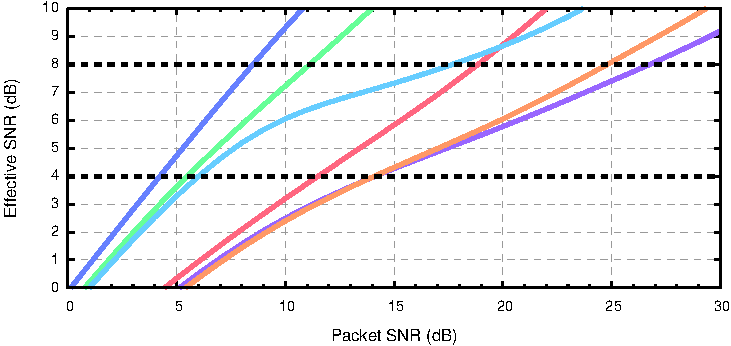
\includegraphics[width=\textwidth]{figures/eff_vs_snr_qpsk.pdf}
  \caption[Effective SNR vs Packet SNR for four faded links]{Effective SNR (for QPSK) versus Packet SNR for flat (left) to faded (right) links.}
  \label{fig:eff_vs_rssi}
\end{figure}

\subsection{Making Predictions with Effective SNR}
I test the ability of Effective SNR to make predictions across power levels by considering the goal of trimming excess transmit power. Excess transmit power is power that can be removed without causing the highest rate for the link to drop.

These experiments start with 88 SISO links from the Intel Labs Testbed configured to radiate 10\mW of transmit power, and a single CSI sample per link. Considering transmit power reductions in increments of 2\dB, the Effective SNR model can predict the best supported rate for each reduced power level, and choose the lower power level with the same best rate. The measurements described earlier include the ground truth packet reception ratio for each power level, and thus these data can be used to check the accuracy of the predictions.

\begin{figure}[t]
      \centering
      \subfigure[Predicted and measured power saving]{%
      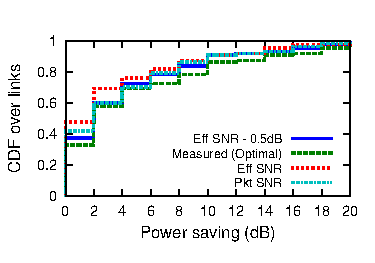
\includegraphics[width=0.5\columnwidth,viewport=0 7 195 110,clip]{figures/power_save_1x1.pdf}%
      \label{fig:power_save_cdf}%
      }%
      \subfigure[Measured PRR corresponding to reduced TX power levels]{%
      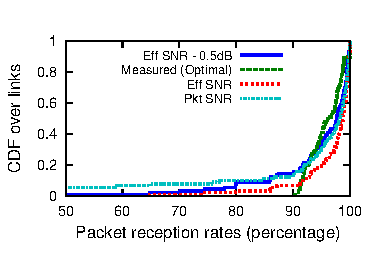
\includegraphics[width=0.5\columnwidth,viewport=0 7 195 110,clip]{figures/power_save_final_prr_1x1.pdf}%
      \label{fig:power_prr_cdf}%
      }%
      \caption[Impact of pruning excess transmit power]{\label{fig:power_save_1x1} Power saving and performance impact of pruning excess transmit power. Pruning with Effective SNR is tight (within 0.5\dB) and does not degrade performance. Pruning with packet SNR degrades performance more without much extra savings.} 
\end{figure}


\figref{fig:power_save_1x1} shows the power savings and performance degradation of four different threshold schemes. A good result here is power savings without a loss of performance; the absolute amount of power savings is not meaningful as it depends on the testbed and the link. The Measured (Optimal) line shows the best that can be done. Measured PRRs at all power levels are used to guide power control decisions. Therefore, the final delivery probabilities are hardly decreased (all links have PRR$\geq$90\%), yet most links save a little power, and some save a lot.

The graphs show that using Effective SNR to predict how much power to trim has a similarly good tradeoff. Impact on rate remains limited, yet power is saved, more than 10\dB for around 10\% of the links. The gap between the Measured and the Eff SNR lines is because Eff SNR thresholds might be slightly conservative for some links.

To show that this trimming is tight, I considered the effect of using more aggressive---i.e. slightly lower (0.5\dB)---Effective SNR thresholds. This operation results in little additional power savings, but degrades performance for many more links.

Finally, I compared this algorithm to a scheme that uses Packet SNR to save power. The results show Packet SNR the savings are barely increased, but more links have degraded performance, and several stop working altogether.

\xxx{@Dan: redo these graphs}

\section{Interference}
\label{sec:interference}
I conclude this chapter by investigating how my Effective SNR-based model can cope with interference. This challenge is one of the largest potential weaknesses of this technique, because Effective SNR is based on measurements taken only during the packet preamble. There are three important components of dealing with interference: 1) maintaining an accurate estimate of interference-free link quality, so that transient interference doesn't cause wild rate swings; 2) recognizing collisions when they occur, to avoid unnecessary rate fallback; and 3) providing an estimate of link quality that enables efficient operation during persistent interference.

I studied the variation of CSI measurements during interference. I chose two nodes at UW that do not detect each other with carrier sense, and alternately designated one as the transmitter and the other as the interferer. The nodes were configured to send large packets designed to collide, while all other receiving nodes monitored the CSI to simulate a total of 20 links. The experiment also varied the transmit power of the node designated as the interferer from low to high to induce a large range of interfering channels, over which I evaluate the impact of interference on CSI measurements and my Effective SNR model.

For all but one of 20 links, the rate predicted by my model for the majority of correct packets was the same with and without interference; the remaining link was off by a single rate. From these measurements, we can conclude that the mere presence of interference does not completely invalidate Effective SNR values, and thus transient interference will not cause wild swings in transmit rate.

To recognize collisions, I propose to leverage a new MAC feature of the 802.11n packet aggregation mechanism. Block ACKs selectively acknowledge frames in a batch of packets transmitted as one continuous burst. Each packet in the burst has a separate checksum, and thus the Block ACK serves as block-based feedback of packet correctness just like the block-based checksums analyzed in PPR~\cite{Jamieson_PPR}. We can therefore use the error patterns in the Block ACK to recognize collisions: when the rate is overselected, errors should be randomly distributed throughout the batch, and bursty when a collision clobbers a continuous part of the batch. The ability to recognize interference and hence decouple interference avoidance and rate selection has been shown to improve performance in many systems (e.g., SoftRate~\cite{Vutukuru_SoftRate}).

Finally, for continuous interference the Effective SNR computed from un-interfered preambles will provide an aggressive estimate, and the system will need another way to compensate. One way to measure the Signal-to-Interference and Noise Ratio (SINR) is to measure the interference as reflected in larger noise floor measurements by the NIC.\footnote{Note that OFDM does not turn interference into inflated RSSI as do the spread spectrum modulations used in 802.11b.} However, the IWL5300 platform does not currently provide this information for dropped packets, and if the interference also experiences fading then this approach may not accurately indicate performance for the same reasons as Packet SNR. An alternative, that I have not yet explored, might be an \define{Effective SINR} metric that incorporates CSI measurements from the interfering nodes to predict packet delivery.

%Because it does not use packet loss as a signal, ESNR will not conservatively reduce rate during interference. Thus transient interference will only cause transient interruptions. However, the Effective SNR measured in a single packet preamble simply does not provide an estimate of link quality when the link experiences persistent interference. One solution is to leverage SoftRate in these circumstances; while Effective SNR can guide the overall choice of antennas and number of spatial streams, SoftRate's continuous estimate of BER may be better suited for choosing rates within one mode. An alternative (that we have not yet explored) might be an \emph{Effective SINR} metric incorporating CSI measurements from the interfering nodes to predict packet delivery.

\section{Summary}
From these results, I conclude that Effective SNR consistently and accurately indicates the best rate for nearly all links and all configurations without any per-link calibration. The low degree of rate confusion with Effective SNR in \secref{sec:rate_confusion} implies that it should be possible to define SNR thresholds that clearly define when a rate will work well. I discuss how to choose these thresholds for practical scenarios in the next chapter. The results in \secref{sec:tx_power_trim} demonstrate the flexibility of this approach by demonstrating that CSI measurements are valid not just across different rates, but also across transmit power scaling. Finally, I showed that Effective SNR measurements are generally not corrupted by transient interference, as long as the packet preamble from which CSI is measured is relatively interference-free.

Having gained confidence that Effective SNR can be useful, in the remainder of this thesis I evaluate Effective SNR at the application level. In the next chapter, I deploy my model as part of a system that selects the optimal rate for a wireless link.

%From now on, we use the thresholds in these graphs to predict the working rate for any link. They agree with the measured SNRs on a wired link (\figref{fig:snr_prr_attenuator}), which strongly suggests that the Effective SNR captures the fundamental error characteristics of the link. 

%%%%%%%%%%%%%%%%%%%%%%%%%%%%%%%%%%
\ifx\mainfile\undefined
%
% ==========   Bibliography   ==========
%
%\nocite{*}   % include everything in the uwthesis.bib file
\bibliographystyle{plain}
\bibliography{dhalperi_thesis}

\end{document}
\fi
